\documentclass[12pt]{article} 
	 
\usepackage{amsmath} 
\usepackage{psfrag,graphicx,verbatim,array,multicol,palatino,enumerate}
\usepackage{amsmath,amsfonts,bm,rotating,natbib}
\usepackage{pstricks,pst-node}
\usepackage{epsfig}
\usepackage{longtable}
\usepackage{graphicx}

\bibliographystyle{natbib}

\textwidth = 6.5in 
\textheight = 9in 
 
\oddsidemargin = -0cm 
 
\evensidemargin = -0.5cm 
 
\parindent 0pt

\parskip 10pt

\topmargin = -1.75cm 
 
\def\balpha{\boldsymbol{\alpha}}
\def\bbeta{\boldsymbol{\beta}}
\def\bmu{\boldsymbol{\mu}}
\def\bsigma{\boldsymbol{\sigma}}
\def\btheta{\boldsymbol{\theta}}
\def\bTheta{\boldsymbol{\Theta}}

\def\bbf{{\bf{f}}}   
\def\bg{{\bf{g}}}   
\def\bm{{\bf{m}}}   
\def\bzero{{\rm {\bf{0}}}}   

\def\bC{{\rm {\bf{C}}}}   
\def\by{{\rm {\bf{y}}}}   
\def\bX{{\rm {\bf{X}}}}   

\begin{document}

\begin{center}
{\large{\bf {\underline{Stat 9270 Homework 1 - Due Friday Feb 7 at 5pm ET}}}}
\end{center}

{\bf You are required to submit a printed pdf document to canvas with answers to the following questions.  Your submitted HW document must be generated using the LaTeX typesetting language. It should also include any requested graphics for each question, integrated with the text for that question. Do not just put all graphics at the end of the document!

Please do all computational work using the software package R. Your R code must be included in your submission as a separate text file. So your homework submission will consist of two files:

1. HW answers in pdf format (created using LaTeX) \\
2. HW code in text format

No late homeworks will be accepted for any reason whatsoever. You should work independently of the other students in the class on each homework.
}

\bigskip

{\underline{\bf Question 1 (10 points)}}  

Let $\theta$ be a random variable that only takes on two values, $\theta = 1$ or 2. If $\theta = 1$, then $y$ has a Normal distribution with mean 1 and standard deviation $\sigma$ whereas if $\theta = 2$, then $y$ has a Normal distribution with mean 2 and standard deviation $\sigma$. Also, suppose $p(\theta = 1) = p(\theta = 2) = 0.5$

(a) For $\sigma = 2$, write the formula for the marginal probability density $p(y)$ and sketch it.

The formula for the marginal probability density $p(y)$ when $\sigma = 2$ is:

\begin{align*}
p(y) &= \sum_{\theta} p(y \, | \, \theta) \cdot p(\theta) \\
p(y) &= \mathcal{N}(1, 2^2) \cdot p(\theta = 1) + \mathcal{N}(2, 2^2) \cdot p(\theta = 2) \\
p(y) &= \mathcal{N}(1, 4) \cdot 0.5 + \mathcal{N}(2, 4) \cdot 0.5 \\
p(y) &= \frac{0.5}{\sqrt{8\pi}} \exp\left( -\frac{(y-1)^2}{8} \right) + \frac{0.5}{\sqrt{8\pi}} \exp\left( -\frac{(y-2)^2}{8} \right)
\end{align*}

A sketch of this marginal probability density $p(y)$ is:

\begin{figure}[h]
    \centering
    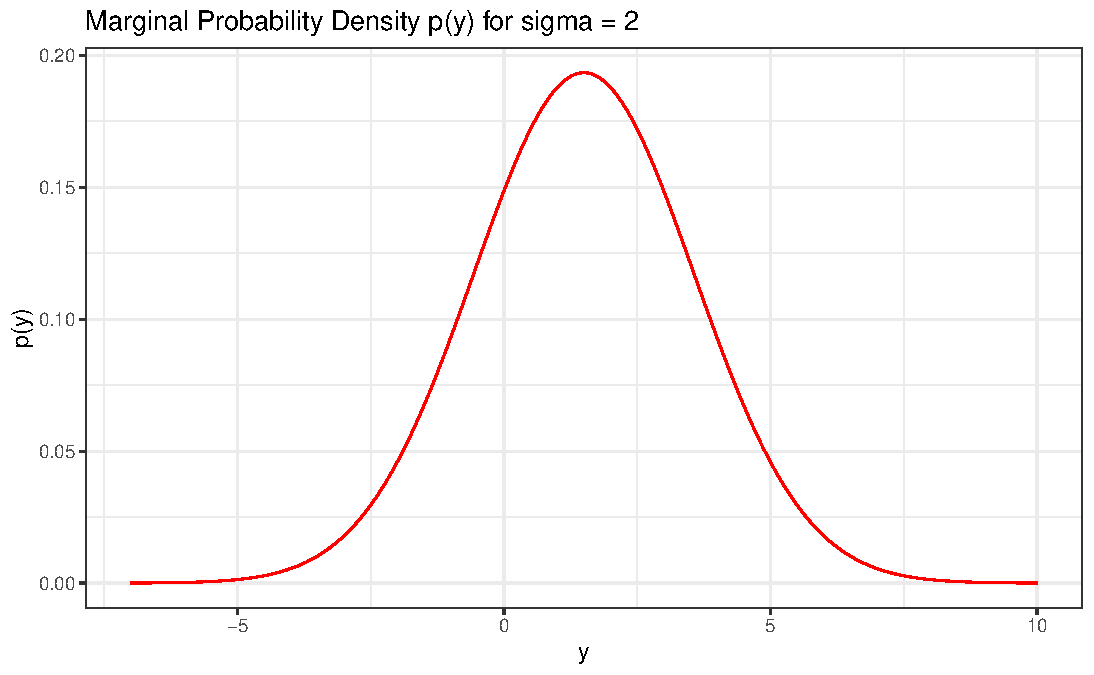
\includegraphics[width=0.7\textwidth]{q1a_plot.pdf}
\end{figure}
\pagebreak

(b) What is $p(\theta = 1 \, | \, y = 1)$, again supposing $\sigma = 2$?

The posterior probability $p(\theta = 1 \, | \, y = 1)$ given $\sigma = 2$ is:

\begin{align*}
p(\theta = 1 \, | \, y = 1) &= \frac{p(y = 1 \, | \, \theta = 1) \cdot p(\theta = 1)}{p(y = 1)} \\
p(\theta = 1 \, | \, y = 1) &= \frac{\frac{1}{\sqrt{8\pi}} \exp\left( -\frac{(1-1)^2}{8}\right) \cdot 0.5}{\frac{0.5}{\sqrt{8\pi}} \exp\left( -\frac{(1-1)^2}{8} \right) + \frac{0.5}{\sqrt{8\pi}} \exp\left( -\frac{(1-2)^2}{8} \right)} \\
p(\theta = 1 \, | \, y = 1) &= \frac{\frac{1}{\sqrt{8\pi}} \exp\left( 0\right) \cdot 0.5}{\frac{0.5}{\sqrt{8\pi}} \exp\left( 0 \right) + \frac{0.5}{\sqrt{8\pi}} \exp\left( -\frac{1}{8} \right)} \\
p(\theta = 1 \, | \, y = 1) &= \frac{\frac{0.5}{\sqrt{8\pi}}}{\frac{0.5}{\sqrt{8\pi}} + \frac{0.5}{\sqrt{8\pi}} \exp\left( -\frac{1}{8} \right)} \\
p(\theta = 1 \, | \, y = 1) &= \frac{\frac{0.5}{\sqrt{8\pi}}\left(1\right)}{\frac{0.5}{\sqrt{8\pi}}\left(1 + \exp\left( -\frac{1}{8} \right)\right) } \\
p(\theta = 1 \, | \, y = 1) &= \frac{1}{1 + \exp\left( -\frac{1}{8} \right)} \\
\end{align*}



(c) Describe how the posterior density of $\theta$ changes in shape as $\sigma$ is increased and as it is decreased.

The posterior distribution takes the form of a sigmoid-like function. This means that the value of $\sigma$ determines
the steepness of the function. As $\sigma$ increases, the exponential term increases more gradually, resulting in a more
gradual transition of the function from 0 to 1.


Conversely, as $\sigma$ decreases, the exponential term grows larger for any given numerator value, which leads to a more
rapid increase in the function from 0 to 1.

By this logic, $\sigma$ acts as a measure of the uncertainty in the posterior distribution of $\theta$, with larger values
of $\sigma$ corresponding to greater uncertainty and more gradual changes in the posterior density of $\theta$.

This is demonstrated below:

\begin{figure}[h]
    \centering
    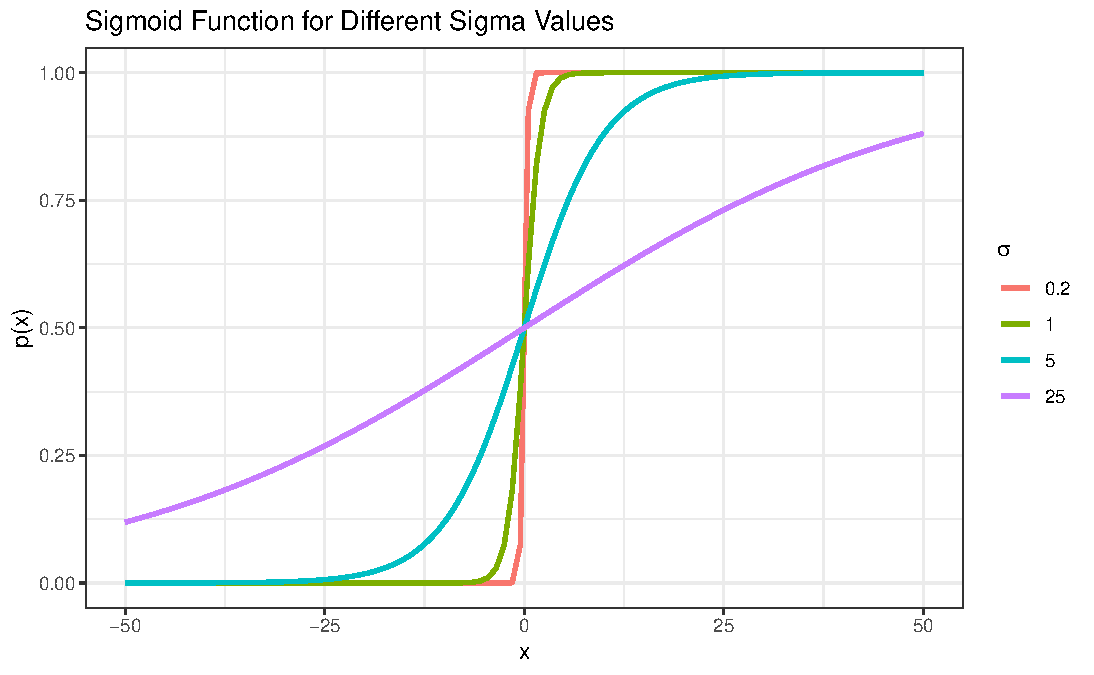
\includegraphics[width=0.7\textwidth]{q1c_plot.pdf}
\end{figure}

\bigskip

{\underline{\bf Question 2 (10 points)}}  

Let $y$ be the number of heads in $n$ coin flips where the probability of heads is $\theta$

(a) If your prior distribution for $\theta$ is Uniform(0,1), then derive the prior predictive
distribution for $y$, i.e.
\begin{eqnarray*}
p(y = k) \, = \, \int\limits_0^1 p(y = k \, | \, \theta) \, {\rm d} \theta  \qquad {\rm for} \quad k = 0,1,\ldots,n
\end{eqnarray*}

Unlike in question 1, we now have a continuous prior distribution for $\theta$, so we need to integrate
over all possible values of $\theta$ to get the prior predictive distribution for $y$, giving us:

$p(y) = \int\limits_0^1 p(y = k \, | \, \theta)p(\theta)d\theta$

Because the prior distribution for $\theta$ is Uniform(0,1), we know $p(\theta) = 1$ for all $\theta \in [0,1]$.
We also know that the Uniform(0,1) prior distribution for $\theta$ is equivalent to a ${\rm Beta}(1,1)$ distribution,
which is conjugate to the binomial likelihood function.

So, we can use conjugacy in our calculation of the probability of observing $k$ heads over all possible values of $\theta$:
\begin{align*}
\int\limits_0^1 p(y = k \, | \, \theta) &= \binom{n}{y}\theta^y\left(1 - \theta\right)^{n-y} p(\theta) d\theta \\
&= \int\limits_0^1 \binom{n}{y}\theta^y\left(1 - \theta\right)^{n-y} \cdot 1 d\theta \\
&= \int\limits_0^1 \binom{n}{y}\theta^y\left(1 - \theta\right)^{n-y}d\theta \\
&= \binom{n}{y} \int\limits_0^1 \theta^y\left(1 - \theta\right)^{n-y}d\theta \\
&= \binom{n}{y} \frac{\Gamma(y + 1) \Gamma(n - y + 1)}{\Gamma(n + 2)} \\
&= \frac{n!}{y!\left(n-y\right)!} \frac{\Gamma(y + 1) \Gamma(n - y + 1)}{\Gamma(n + 2)} \\
&= \frac{\Gamma(n+1)}{\Gamma(y+1)\Gamma(n-y+1)} \frac{\Gamma(y + 1) \Gamma(n - y + 1)}{\Gamma(n + 2)} \\
&= \frac{\Gamma(n+1)}{\Gamma(n + 2)} \\
&= \frac{\Gamma(n+1)}{(n + 1)\Gamma(n + 1)} \\
&= \frac{1}{n + 1} \\
\end{align*}

So the prior predictive distribution for $y$ is $p(y) = \frac{1}{n + 1}$ for $y = 0,1,\ldots,n$, which is a Uniform distribution as it's not dependent on anything but $n$. As we would expect, when we take advantage of the conjugacy of the Uniform(0,1) prior distribution for $\theta$ with the binomial likelihood function,
we find that the prior predictive distribution for $y$ is Uniform.

(b) Suppose you assign a ${\rm Beta}(a, b)$ prior distribution for $\theta$, and then you observe $y
$ heads out of $n$ coin flips.  Show algebraically that the posterior mean of $\theta$ always lies between the prior mean $a/(a+b)$ and the observed proportion of heads $y/n$.

With a ${\rm Beta}(a, b)$ prior distribution for $\theta$, $p(\theta | y) \sim \rm Beta(y + a, n - y + b)$,
which gives a posterior mean of: $E(\theta | y) = \frac{y + a}{n + a + b}$.

We can show that this posterior mean always lies between the prior mean $a/(a+b)$ and the observed proportion of heads $y/n$ by proving that either
$\frac{a}{a + b} \leq \frac{y + a}{n + a + b} \leq \frac{y}{n}$ when $\frac{a}{a + b} \leq \frac{y}{n}$
or $\frac{a}{a + b} \geq \frac{y + a}{n + a + b} \geq \frac{y}{n}$ when $\frac{a}{a + b} \geq \frac{y}{n}$. Because these proofs are just the inverse of each other,
we will proceed with the first case, where we assume $\frac{a}{a + b} \leq \frac{y}{n}$.

First, we will show that if $\frac{a}{a + b} \leq \frac{y}{n}$, then $\frac{a}{a + b} \leq \frac{y + a}{n + a + b}$. Starting with the given inequality assumption:

\begin{align*}
\frac{a}{a + b} &\leq \frac{y}{n} \\
an &\leq ya + yb \\
\end{align*}

And then looking at the target inequality:

\begin{align*}
\frac{a}{a + b} &\leq \frac{y + a}{n + a + b} \\
a\left(n+ a + b\right) &\leq \left(y + a\right)\left(a + b\right) \\
an + a^2 + ab &\leq ya + yb + a^2 + ab \\
an &\leq ya + yb \\
\end{align*}

So, we see that if $\frac{a}{a + b} \leq \frac{y}{n}$, then $\frac{a}{a + b} \leq \frac{y + a}{n + a + b}$.

Now we want to show that if $\frac{a}{a + b} \leq \frac{y}{n}$, then $\frac{y + a}{n + a + b} \leq \frac{y}{n}$. Starting with the given inequality assumption:

Looking at the target inequality:

\begin{align*}
\frac{y + a}{n + a + b} &\leq \frac{y}{n} \\
n\left(y + a\right) &\leq y\left(n + a + b\right) \\
yn + an &\leq yn + ya + yb \\
an &\leq ya + yb \\
\end{align*}

Now we see that the three inequalities, our given assumption, $\frac{a}{a + b} \leq \frac{y}{n}$,
and the two target inequalities, $\frac{a}{a + b} \leq \frac{y + a}{n + a + b}$ and $\frac{y + a}{n + a + b} \leq \frac{y}{n}$,
are all equivalent. This means that the posterior mean of $\theta$ always lies between the prior mean $a/(a+b)$ and the observed
proportion of heads $y/n$.

(c) Show that if the prior distribution on $\theta$ is uniform, then the posterior variance of $\theta$ is always less than the prior variance.

This statement makes intuitive sense, as a uniform prior on $\theta$ considers all values of $\theta$ equally likely, and therefore maximizes
the prior variance of $\theta$. When we observe data and update our prior distribution to a posterior distribution, we are effectively reducing
the uncertainty in our estimate of $\theta$, which means that the posterior variance of $\theta$ will be less than the prior variance.

We can show this algebraically by calculating the prior and posterior variances of $\theta$ when the prior distribution of
$\theta$ is Uniform(0,1) and comparing them. For a Uniform(0,1) prior distribution, the prior variance of $\theta$ is equal
to the variance of a $\rm Beta(1,1)$ distribution, the formula of which is: $Var(\theta) = \frac{1 \cdot 1}{(1 + 1)^2(1 + 1 + 1)} = \frac{1}{12}$.

We showed above in part (a) that the posterior distribution of $\theta$ given $y$ is $\rm Beta(y + 1, n - y + 1)$, which has a variance of:
$Var(\theta | y) = \frac{(y + 1)(n - y + 1)}{(n + 2)^2(n + 3)}$. 

We can compare the prior and posterior variances of $\theta$ by showing that $Var(\theta | y) < Var(\theta)$:

\begin{align*}
\frac{(y + 1)(n - y + 1)}{(n + 2)^2(n + 3)} &< \frac{1}{12} \\
12(y + 1)(n - y + 1) &< (n + 2)^2(n + 3) \\
(12y + 12)(n - y + 1) &< (n^2 + 4n + 4)(n + 3) \\
12yn - 12y^2 + 12n + 12 &< n^3 + 7n^2 + 16n + 12 \\
\end{align*}

From this we can see that for any values of $y \geq 1$ and $n \geq 1$, the above inequality will hold,
which means that the posterior variance of $\theta$ is always less than the prior variance when 
the prior distribution on $\theta$ is uniform.

To make this even more clear we can plug in y = 1 and n = 1 to show that the inequality holds:

\begin{align*}
12(1) - 12(1) + 12 + 12 &< 1 + 7 + 16 + 12 \\
24 &< 36 \\
\end{align*}

and y = 1 and n = 2 to show that the difference between the left and right-hand sides only grows as n increases:

\begin{align*}
12(1)(2) - 12(1)^2 + 12(2) + 12 &< 2^3 + 7(2)^2 + 16(2) + 12 \\
48 &< 80 \\
\end{align*}


(d) Give an example of a ${\rm Beta}(a, b)$ prior distribution and data $(y,n)$ for which the posterior
variance of $\theta$ is higher than the prior variance.

To achieve this example we want our prior distribution for $\theta$ to have a very low variance
and our data to be such that the posterior distribution of $\theta$ has a very high variance. The formula for the
prior variance of $\theta$ is $Var(\theta) = \frac{a \cdot b}{(a + b)^2(a + b + 1)}$, so to minimize the prior variance,
we want imbalanced values of $a$ and $b$ that are large when summed, as the denominator grows cubically
on $a + b$. We can set these values to $a = 1$ and $b = 100$, which gives us a prior variance of:

$Var(\theta) = \frac{100}{(101)^2(102)} = \frac{100}{1040502} = 0.000096107$.

Now we can choose data $(y,n)$ such that the posterior distribution of $\theta$ has a large variance. Again, the formula
for the posterior variance of $\theta$ when $a = 1$ and $b = 100$ is:

$Var(\theta | y) = \frac{(y + a)(n - y + b)}{(n + a + b)^2(n + a + b + 1)} = \frac{(y + 1)(n - y + 100)}{(n + 101)^2(n + 102)}$.

So, we want a small value of $n$ relative to $y$ to maximize the posterior variance of $\theta$. 

We can choose $y = 1$ and $n = 2$:

$Var(\theta | y) = \frac{(1 + 1)(2 - 1 + 100)}{(2 + 101)^2(2 + 102)} = \frac{202}{103^2 \cdot 104} = \frac{202}{1103336} = 0.000183081$.

And $0.000183081 > 0.000096107$, so we have found an example where the posterior variance of $\theta$ is greater than the prior
variance of $\theta$ using a prior distribution of ${\rm Beta}(1, 100)$ and data $(1, 2)$.

\bigskip

{\underline{\bf Question 3 (10 points)}}  

Suppose your prior distribution for $\theta$, the proportion of Californians who support the death penalty, is a Beta distribution with mean of 0.6 and standard deviation of 0.3

(a) Determine the hyper-parameters $a$ and $b$ for a ${\rm Beta} (a,b)$ prior distribution with mean of 0.6 and standard deviation of 0.3.  Plot the prior density function.

For a beta distribution, the mean and standard deviation are given by:

Mean: $\mu = \frac{a}{a + b}$

Standard Deviation: $\sigma = \sqrt{\frac{ab}{(a+b)^2(a+b+1)}}$

We can solve these equations to find the hyper-parameters $a$ and $b$ for a ${\rm Beta} (a,b)$ prior distribution with mean of 0.6 and standard deviation of 0.3:

\begin{align*}
0.6 &= \frac{a}{a + b} \\
0.3 &= \sqrt{\frac{ab}{(a+b)^2(a+b+1)}} \\
\end{align*}

We can start by solving for $b$ in the first equation:

\begin{align*}
0.6(a + b) &= a \\
0.6a + 0.6b &= a \\
0.6b &= 0.4a \\
b &= \frac{2}{3}a \\
\end{align*}

Now we can substitute this value of $b$ into the second equation:

\begin{align*}
0.3 &= \sqrt{\frac{a\left(\frac{2}{3}a\right)}{(a + \frac{2}{3}a)^2(a + \frac{2}{3}a + 1)}} \\
0.3 &= \sqrt{\frac{\frac{2}{3}a^2}{\left(\frac{5}{3}a\right)^2\left(\frac{5}{3}a + 1\right)}} \\
0.3 &= \sqrt{\frac{\frac{2}{3}a^2}{\frac{25}{9}a^2\left(\frac{5}{3}a + 1\right)}} \\
0.3 &= \sqrt{\frac{\frac{2}{3}}{\frac{25}{9}\left(\frac{5}{3}a + 1\right)}} \\
0.3 &= \sqrt{\frac{6}{25\left(\frac{5}{3}a + 1\right)}} \\
0.3 &= \frac{\sqrt{6}}{5\sqrt{\frac{5}{3}a + 1}} \\
1.5 &= \frac{\sqrt{6}}{\sqrt{\frac{5}{3}a + 1}} \\
1.5^2 &= \frac{6}{\frac{5}{3}a + 1} \\
2.25 &= \frac{6}{\frac{5}{3}a + 1} \\
2.25\left(\frac{5}{3}a + 1\right) &= 6 \\
\frac{27}{12} \cdot \frac{20}{12}a + 2.25 &= 6 \\
\frac{540}{144}a &= 3.75 \\
a &= 3.75 \cdot \frac{144}{540} \\
a &= 1 \\
\end{align*}

and

\begin{align*}
b &= \frac{2}{3}a \\
b &= \frac{2}{3} \\
\end{align*}

We can visualize this prior density function with the following plot:

\begin{figure}[h]
    \centering
    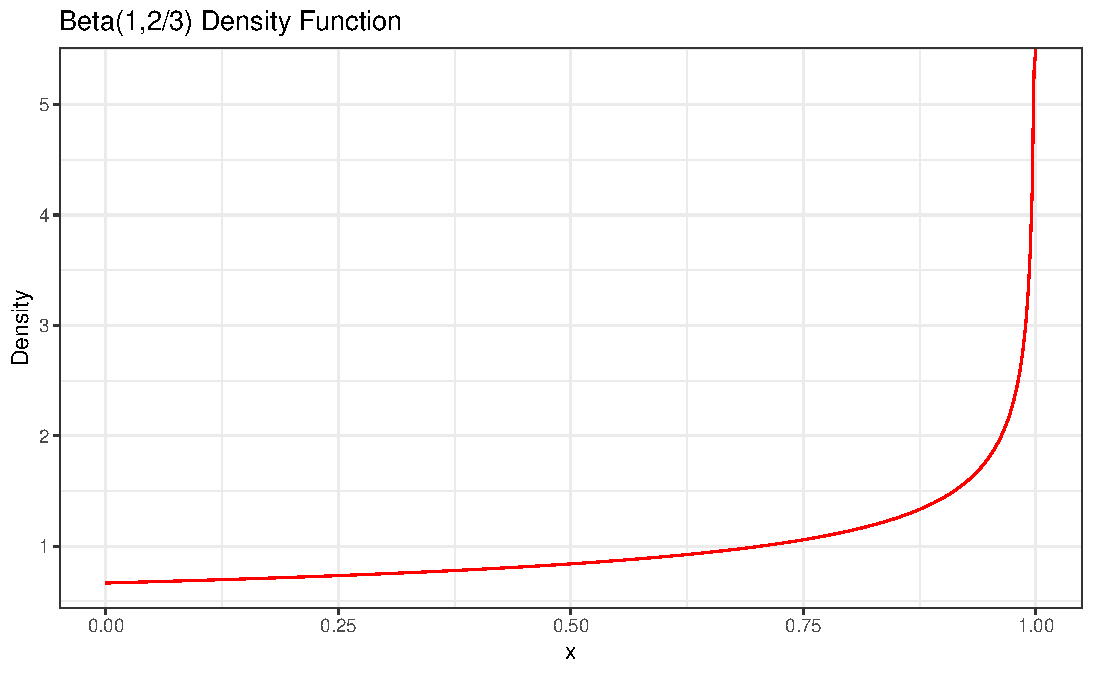
\includegraphics[width=0.7\textwidth]{q3a_plot.pdf}
\end{figure}

(b) A random sample of 1000 Californians is taken, and 65\% support the death penalty.  What is the posterior mean and variance for $\theta$? Draw the posterior density function $p(\theta \, | \, y)$

The likelihood function for the data is given by the binomial distribution. This means that we can take advantage of 
conjugacy between the Beta prior distribution and the binomial likelihood function, giving us a Beta posterior distribution 
of $p(\theta \, | \, y) = {\rm Beta}(y + a, n - y + b)$ with posterior mean of $E(\theta | y) = \frac{y + a}{n + a + b}$ and
posterior variance of $Var(\theta | y) = \frac{(y + a)(n - y + b)}{(n + a + b)^2(n + a + b + 1)}$.

In this case, $y = 650$, $n = 1000$, $a = 1$, and $b = \frac{2}{3}$, so the posterior mean for $\theta$ is:

\begin{align*}
E(\theta | y) &= \frac{650 + 1}{1000 + 1 + \frac{2}{3}} \\
&= \frac{651}{1001\frac{2}{3}} \\
&= 0.649916805 \\
\end{align*}

and the posterior variance for $\theta$ is:

\begin{align*}
Var(\theta | y) &= \frac{(650 + 1)(1000 - 650 + \frac{2}{3})}{(1000 + 1 + \frac{2}{3})^2(1000 + 1 + \frac{2}{3} + 1)} \\
&= \frac{651 \cdot 350\frac{2}{3}}{(1001\frac{2}{3})^2(1002\frac{2}{3})} \\
&= \frac{228284}{1003336.11111 \cdot 1002\frac{2}{3}} \\
&= \frac{228284}{1006011674.074074} \\
&= 0.00022692 \\
\end{align*}


Lastly, we can visualize this posterior density function, $p(\theta \, | \, y) = {\rm Beta}(y + a, n - y + b) = {\rm Beta}(651, 350\frac{2}{3})$,
with the following plot:

\begin{figure}[h]
    \centering
    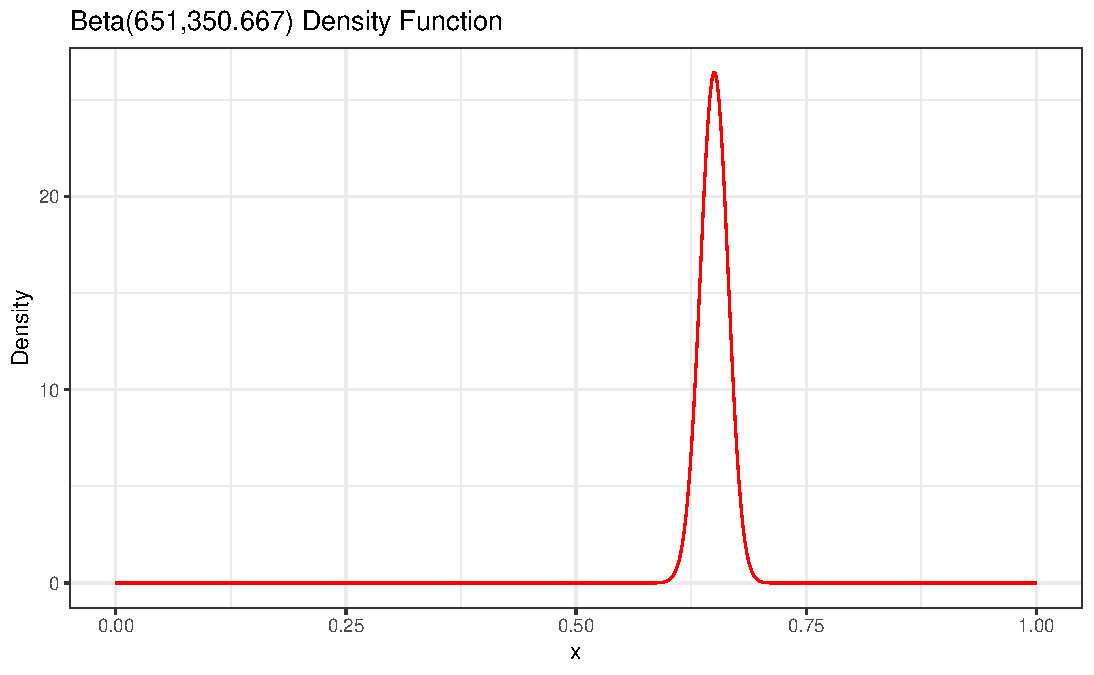
\includegraphics[width=0.7\textwidth]{q3b_plot.pdf}
\end{figure}

\bigskip

{\underline{\bf Question 4 (10 points)}}  

We have observations $(y_1,\ldots,y_5) = (43, 44, 45, 46.5, 47.5)$ which are independent samples from a Cauchy distribution with unknown center $\theta$ and known scale 1, which has a probability density of 
\begin{eqnarray*}
p(y_i \, | \, \theta) \, \propto \, \frac{1}{1 + (y_i - \theta)^2} 
\end{eqnarray*}
Assume that the prior distribution for $\theta$ is Uniform on [0, 100].  

(a) Calculate the unnormalized posterior density function, $p(\theta | \by)$ on an evenly-spaced grid of 1000 points in the interval [0, 100] and plot that posterior density function $p(\theta | \by)$

The unnormalized posterior density function is given by:

\begin{align*}
p(\theta | \by) &\propto p(\by | \theta) \cdot p(\theta) \\
&\propto \prod_{i=1}^5 \frac{1}{1 + (y_i - \theta)^2} \cdot 1 \\
&\propto \frac{1}{1 + (43 - \theta)^2} \cdot \frac{1}{1 + (44 - \theta)^2} \cdot \frac{1}{1 + (45 - \theta)^2} \cdot \frac{1}{1 + (46.5 - \theta)^2} \cdot \frac{1}{1 + (47.5 - \theta)^2} \\
\end{align*}

Using this formula, we can calculate the unnormalized posterior density function on an evenly-spaced grid of 1000 points in
the interval [0, 100] in R and visualize the resulting posterior density function:

\begin{figure}[h]
    \centering
    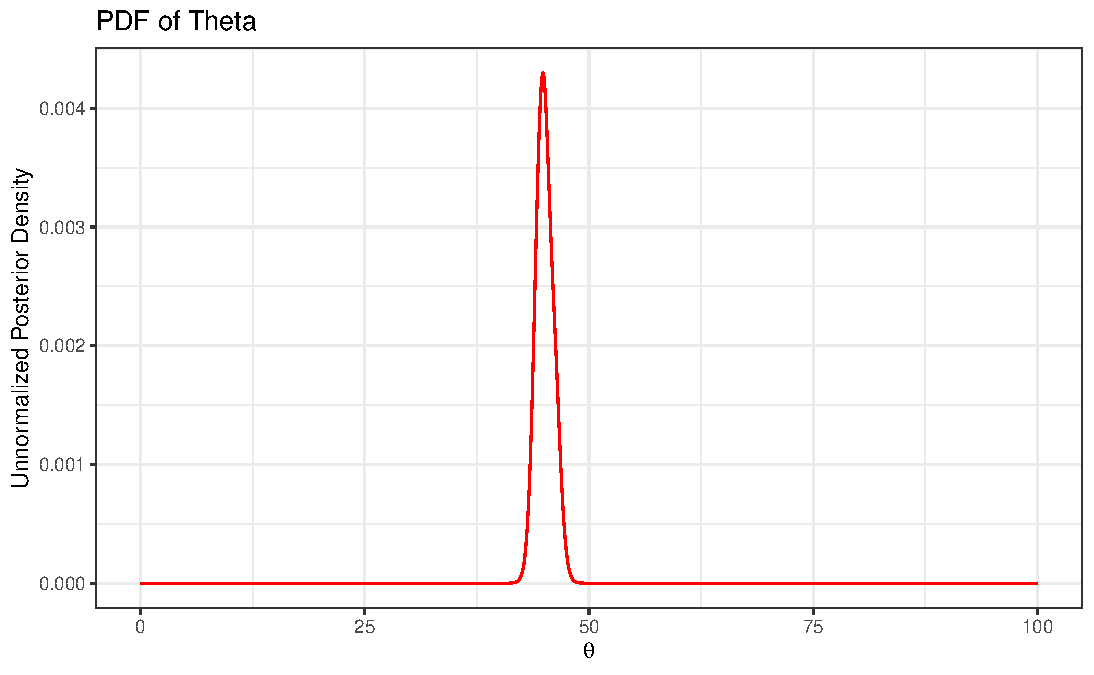
\includegraphics[width=0.7\textwidth]{q4a_plot.pdf}
\end{figure}

(b) Sample 1000 samples of $\theta$ from the posterior density and plot a histogram of those samples

The sampling and visualization was performed in R, with the resulting plot shown below:

\begin{figure}[h]
    \centering
    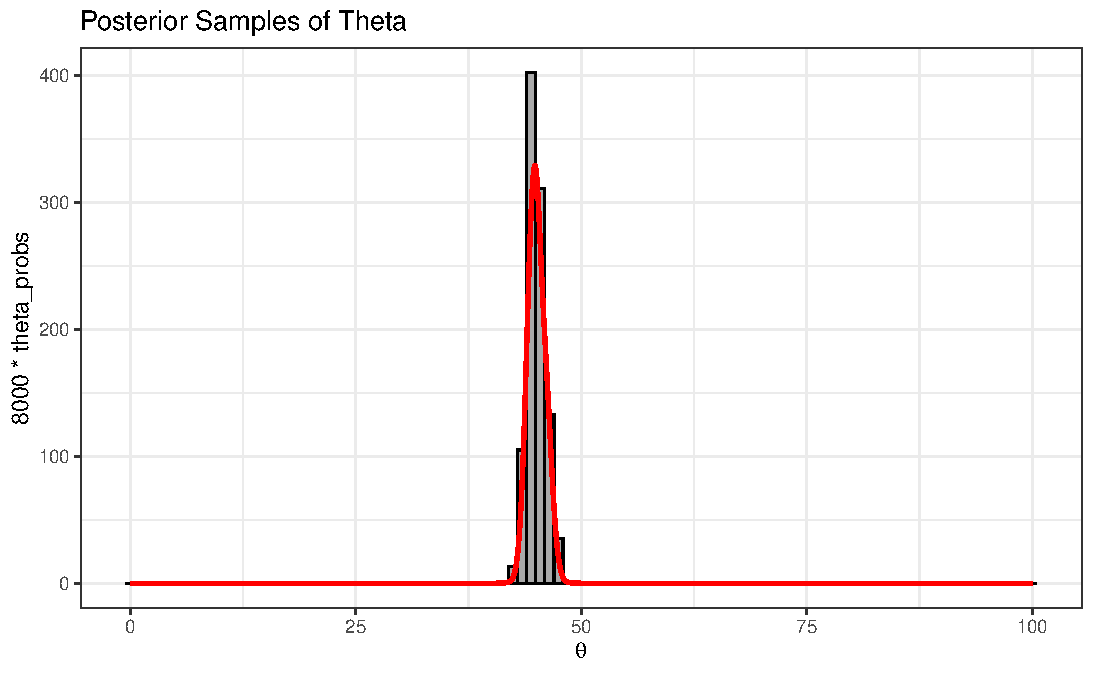
\includegraphics[width=0.7\textwidth]{q4b_plot.pdf}
\end{figure}

\pagebreak

(c) Use those 1000 samples of $\theta$ to obtain 1000 samples from the predictive distribution of a future observation, $y_6$, and plot a histogram of those predictive samples

The predictive distribution of a future observation, $y_6$, is given by:

\begin{align*}
p(y_6 | \by) &= \int p(y_6 | \theta) \cdot p(\theta | \by) d\theta \\
&= \int \frac{1}{1 + (y_6 - \theta)^2} \cdot p(\theta | \by) d\theta \\
\end{align*}

Using the 1000 samples of $\theta$ from the posterior density, we can generate 1000 samples from the predictive distribution of $y_6$ by sampling from the Cauchy distribution with each sampled $\theta$ as the location parameter.

The sampling and visualization was performed in R, with the resulting plot shown below:

\begin{figure}[h]
    \centering
    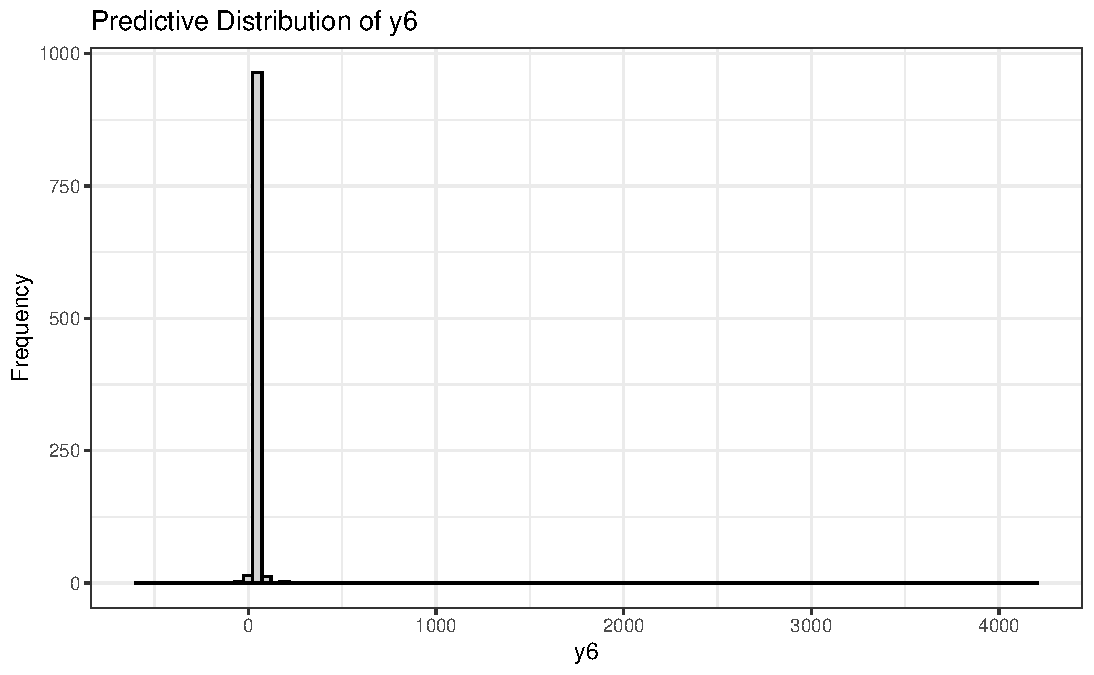
\includegraphics[width=0.7\textwidth]{q4c_plot.pdf}
\end{figure}

\pagebreak

{\underline{\bf Question 5 (10 points)}}  

Suppose $y$ has a binomial distribution for given $n$ and unknown parameter $\theta$ where the prior distribution for $\theta$ is ${\rm Beta} (a,b)$

(a) Find $p(y)$, the marginal distribution of for $y = 0, . . . , n$ (integrating over $\theta$).  This discrete distribution is known as the {\it beta-binomial}

The marginal distribution of $y$ is given by:
$\int\limits_0^1 p(y | \theta)p(\theta) d\theta$, as the possible values of $\theta$ with a Beta 
prior distribution are continuous on the interval [0,1].

We know that p($y | \theta$) is given by the binomial distribution, $p(y | \theta) = \binom{n}{y}\theta^y(1 - \theta)^{n-y}$, and
that p($\theta$) is given by the Beta distribution, $p(\theta) = \frac{\theta^{a-1}(1 - \theta)^{b-1}}{B(a,b)}$, so:

\begin{align*}
p(y) = \int\limits_0^1 p(y | \theta)p(\theta) d\theta &= \int\limits_0^1\binom{n}{y}\theta^y(1 - \theta)^{n-y}\frac{\theta^{a-1}(1 - \theta)^{b-1}}{B(a,b)}d\theta \\
&= \binom{n}{y}\frac{1}{B(a,b)}\int\limits_0^1\theta^{y + a - 1}(1 - \theta)^{n - y + b - 1}d\theta \\
&= \binom{n}{y}\frac{1}{B(a,b)}B(y + a, n - y + b) \\
&= \binom{n}{y}\frac{B(y + a, n - y + b)}{B(a,b)} \\
\end{align*}

So, the marginal distribution of $y$ is the beta-binomial distribution, $p(y) = \binom{n}{y}\frac{B(y + a, n - y + b)}{B(a,b)}$.

(b) Show that if the beta-binomial probability $p(y)$ is constant in $y$ then the prior distribution has to have $a = b = 1$

For the beta-binomial probability $p(y)$ to be constant in $y$, we cannot have any dependence on $y$ in the beta-binomial distribution.
This means that when we expand out the beta-binomial distribution, the terms that depend on $y$ must cancel out, leaving only the terms that depend on $n$:

\begin{align*}
p(y) &= \binom{n}{y}\frac{B(y + a, n - y + b)}{B(a,b)} \\
&= \binom{n}{y}\frac{\Gamma(y + a)\Gamma(n - y + b)}{\Gamma(y + a + n - y + b)}\frac{\Gamma(a + b)}{\Gamma(a) + \Gamma(b)} \\
&= \binom{n}{y}\frac{\Gamma(y + a)\Gamma(n - y + b)}{\Gamma(a + n + b)}\frac{\Gamma(a + b)}{\Gamma(a) + \Gamma(b)} \\
&= \frac{\Gamma(n+1)}{\Gamma(y+1)\Gamma(n-y+1)}\frac{\Gamma(y + a)\Gamma(n - y + b)}{\Gamma(a + n + b)}\frac{\Gamma(a + b)}{\Gamma(a) + \Gamma(b)} \\
\end{align*}

As we can see, the terms that depend on $y$, $\Gamma(y+1)\Gamma(n-y+1)$ and $\Gamma(y + a)\Gamma(n - y + b)$, only cancel out
when $a = b = 1$. To demonstrate:

\begin{align*}
Given \, a = b = 1: \\
p(y) &= \frac{\Gamma(n+1)}{\Gamma(y+1)\Gamma(n-y+1)}\frac{\Gamma(y + 1)\Gamma(n - y + 1)}{\Gamma(n + 2)}\frac{\Gamma(2)}{\Gamma(1) + \Gamma(1)} \\
&= \frac{\Gamma(n+1)}{\Gamma(n+2)}\frac{\Gamma(2)}{\Gamma(1) + \Gamma(1)} \\
\end{align*}

And now the beta-binomial probability, $p(y)$, is constant in $y$ because the terms that depend on $y$ have
canceled out. We've shown this only occurs when the prior distribution has $a = b = 1$.

\bigskip


{\underline{\bf Question 6 (10 points)}}  

Our airline crash dataset ({\bf planes.txt: posted on canvas}) gives the number of fatal accidents and deaths on scheduled airline flights per year over a ten-year period from 1976 through 1985.  Assume that the numbers of fatal accidents $y_t$ in each year $t$ follows a Poisson distribution with mean $\alpha + \beta \cdot t$. 

(a) Choose a noninformative prior for $(\alpha, \beta)$ and use grid sampling to obtain 1000 samples of $(\alpha, \beta)$ from their joint posterior distribution.  Give a 2D contour plot of the joint posterior distribution evaluated over your grid of values

For a likelihood function given by the Poisson distribution, we have a few options we can choose from if we want
to use a noninformative prior. In this case we will use a flat prior, which means $p(\alpha, \beta) \propto 1$.
This gives us a joint posterior distribution of:

Given a flat prior $p(\alpha, \beta) \propto 1$, the joint posterior distribution of $\alpha$ and $\beta$ is given by:
\begin{align*}
p(\alpha, \beta | y) &\propto p(y | \alpha, \beta) \cdot p(\alpha, \beta) \\
&\propto p(y | \alpha, \beta) \cdot 1 \\
&\propto p(y | \alpha, \beta) \\
&\propto \prod_{t=1}^{10} \frac{(\alpha + \beta t)^{y_t}e^{-(\alpha + \beta t)}}{y_t!} \\
&\propto \prod_{t=1}^{10} (\alpha + \beta t)^{y_t}e^{-(\alpha + \beta t)} \\
\end{align*}

The grid sampling was performed in R, with the resulting 2D contour plot of the joint posterior distribution shown below:

\begin{figure}[h]
    \centering
    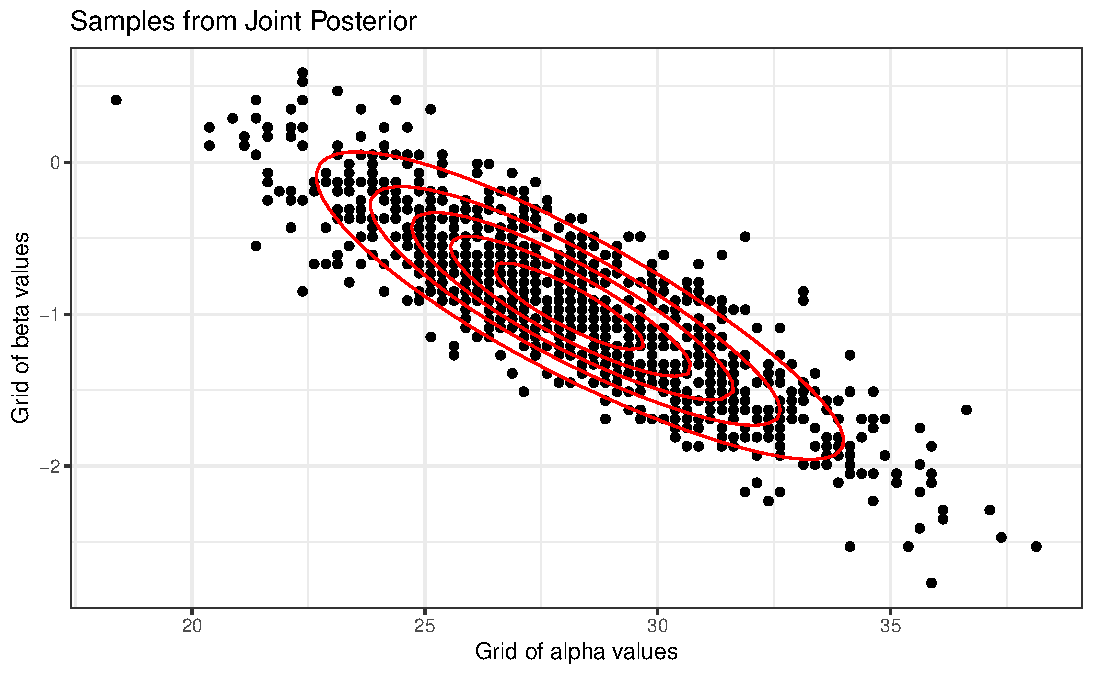
\includegraphics[width=0.7\textwidth]{q6a_plot.pdf}
\end{figure}

(b) Use the samples from (b) to obtain 1000 samples from the posterior predictive distribution for $y^\star$,
the number of fatal accidents in 1986.  Plot a histogram and calculate a 95\% posterior predictive interval
for the number of fatal accidents in 1986. 

The code for sampling, visualization, and calculating a 95\% posterior predictive interval are included in
the associated R file. The histogram with the boundaries of the 95\% posterior predictive interval marked
by red lines is shown below:

\begin{figure}[h]
    \centering
    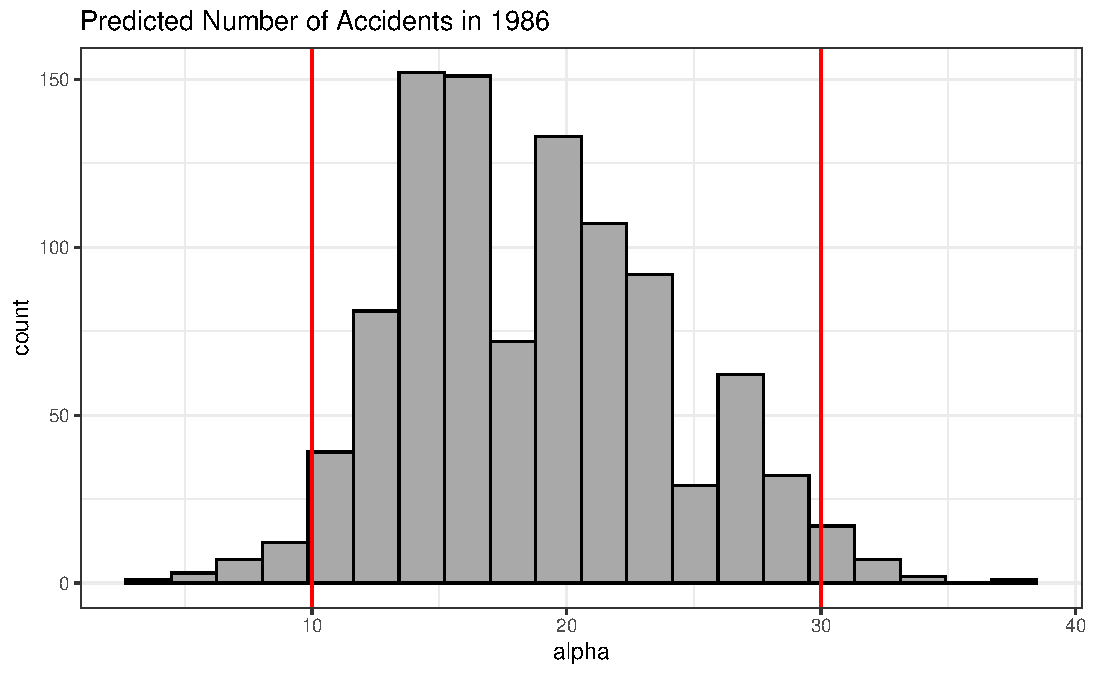
\includegraphics[width=0.7\textwidth]{q6b_plot.pdf} \\
\end{figure}


\pagebreak

{\underline{\bf Question 7 (20 points)}}  

A clinic has three doctors. Starting at 9 am, patients come into the clinic at random times: the time after opening at which the first patient appears follows an exponential distribution with expectation 10 minutes and then, after each patient arrives, the waiting time until the next patient is independently exponentially distributed, also with expectation 10 minutes.   When a patient arrives, he or she waits until a doctor is available. The amount of time spent by each doctor with each patient is also a random variable, uniformly distributed between 5 and 20 minutes. The office stops admitting new patients at 4 p.m. and closes when the last patient is through with their doctor.

(a) Simulate this process once. How many patients came to the office? How many had to wait for a doctor? What was their average wait? When did the office close?

Before we can simulate this process, we need to understand each of the components that make up the process. We know that the
arrivals of patients follow exponential distributions with expectation 10 minutes. The office admits new patients from 9 am
to 4 pm, which is a total of 7 hours or 420 minutes. We can simulate the arrival of patients by generating random exponential
variables with $\lambda = 1/10$ until the total time exceeds 420 minutes. This simulation will give us the arrival times
for each patient, which will allow us to determine how many patients came to the office.

The duration of each doctor visit is uniformly distributed between 5 and 20 minutes. There are three doctors, so the first
three patients will be seen immediately. After the first three patients, we will need to track when each doctor becomes 
available, so that we can assign new patients to the earliest available doctor. If a patient must wait, their wait time will
be recorded as the difference between their arrival time and the time when a doctor becomes available.

Lastly, the office will close once the last patient to arrive before 4pm has finished their visit with a doctor.

The code for simulating this process a single time is included in the associated R file. 
The simulation results are as follows:

\begin{itemize}
\item Number of patients who came to the office: 43
\item Number of patients who had to wait for a doctor: 4
\item Average wait time: 3.49489207116044 minutes
\item Office closed at: 4:05pm
\end{itemize}

(b) Simulate the process 100 times and estimate the median and a 95\% interval for each of the four quantities calculated in (a)

The code for simulating this process 100 times and calculating the median and 95\% interval for each of the four quantities
is included in the associated R file. The results are as follows:

\begin{itemize}
\item Median number of patients who came to the office: 41
\item 95\% interval for number of patients who came to the office: [32, 54]
\item Median number of patients who had to wait for a doctor: 5
\item 95\% interval for number of patients who had to wait for a doctor: [0, 15]
\item Median average wait time: 3.52926889792718 minutes
\item 95\% interval for average wait time: [0 minutes, 7.45380334304729 minutes]
\item Median office closing time: 4:08pm
\item 95\% interval for office closing time: [3:35pm, 4:19pm]
\end{itemize}

\bigskip

{\underline{\bf Question 8 (20 points)}}  

In this exercise, your goal is simulate the distribution of the number of runs scored by a batting lineup in a single inning of baseball.  In baseball, batters try to get on base via various types of hits.  If they get on base, batters are called runners and they try to score by sequentially advancing through the bases. 

We will consider a simplified version of baseball where there are only four outcomes for each batter:
\begin{enumerate} 
\item Out: outs increase by 1, no runners advance, no runs scored
\item Single: batter becomes runner at first base, current runners advance one base with runner on 3rd base scoring
\item Double: batter becomes runner at second base, current runners advance two bases with runners on 2nd and 3rd scoring
\item Home run: batter and any current runners score, bases are emptied of runners
\end{enumerate}

For simplicity, we will also assume that each batter in the batting lineup has the same outcome probabilities: 
\begin{eqnarray*}
P(out)  =  0.65, P(single)  =  0.2, P(double)  =  0.1, P(homerun)  =  0.05
\end{eqnarray*}

In this simulation, you will need to randomly sample the outcome for each batter as well as track and update any runners on the three bases as well as the number of runs scored or if an out was recorded.  The inning continues until three outs are sampled, and then the total number of runs scored is the output of that simulated inning.

(a) Code up the simulation described above and use it to generate the distribution of the number of runs scored in each of 1000 simulated innings.  Provide a histogram and 95\% posterior interval for the distribution the number of runs scored in a 3-out inning.  

The code for simulating the distribution of the number of runs scored in each of 1000 simulated 3-out innings
is included in the associated R file. The histogram for the distribution of the number of runs scored,
with 95\% posterior intervals in red, is shown below:

\begin{figure}[h]
    \centering
    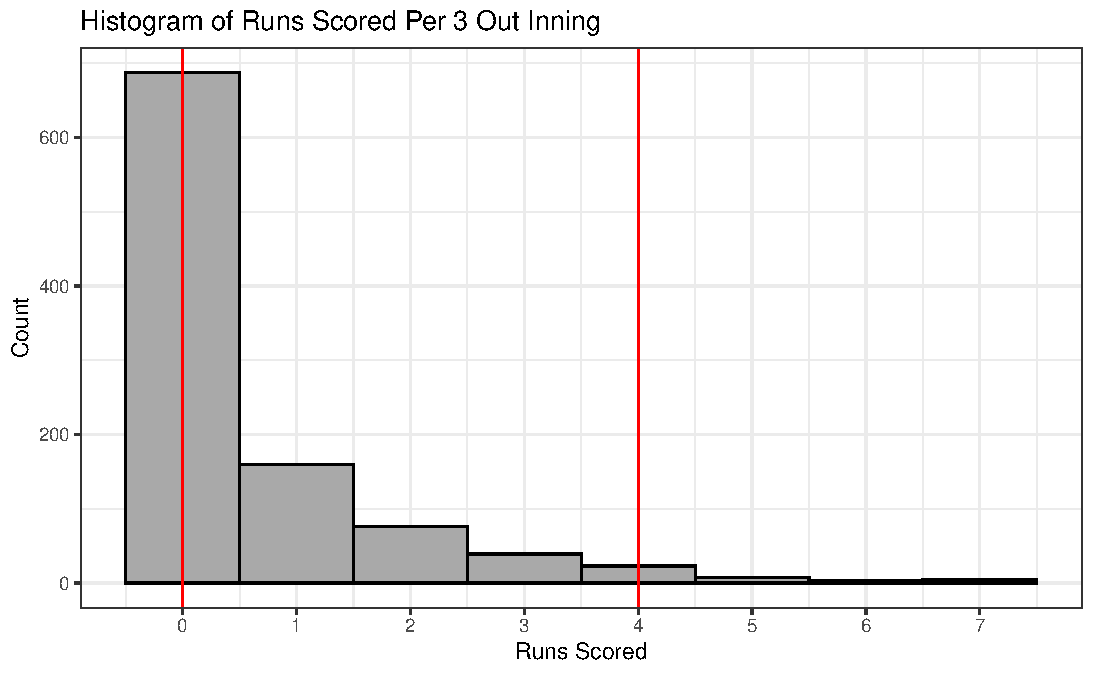
\includegraphics[width=0.7\textwidth]{q8a_plot.pdf}
\end{figure}

(b) Now consider the unusual situation where the defending team makes a series of fielding blunders that result in the batting team getting 6 outs in their inning instead of 3 outs.  Use the same simulation assumptions above to generate the distribution of the number of runs scored in each of 1000 simulated innings that now consist of 6 outs instead of 3.   Provide a histogram and 95\% posterior interval for the distribution the number of runs scored in a 6-out inning.  

The code for simulating the distribution of the number of runs scored in each of 1000 simulated 6-out innings
is included in the associated R file. The histogram for the distribution of the number of runs scored,
with 95\% posterior intervals in red, is shown below:

\begin{figure}[h]
    \centering
    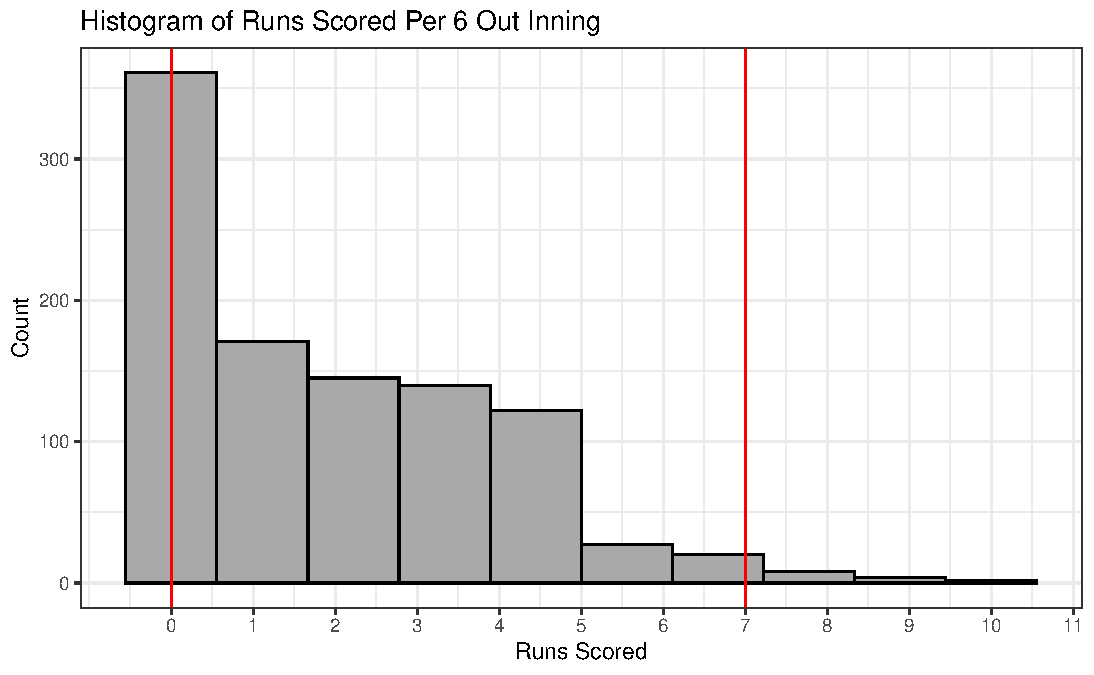
\includegraphics[width=0.7\textwidth]{q8b_plot.pdf}
\end{figure}

{\underline{\bf Generative AI}}  

Throughout the completion of this homework, VSCode with integrated GitHub CoPilot was used
to generate the LaTeX document. Additionally, OpenAI's ChatGPT, Anthropic's Claude, and DeepSeek were 
used to validate answers and check R code for correctness, often resulting in refinements of both written
answers and code implementation.

\end{document}

